\section{並查集}
    \subsection{前言}
    並查集又稱為DSU(Disjoint Set Union),顧名思義就是專門處理合併與查詢集合的資料結構。
    
    我們常常會遇到這樣的問題,兩個人是否同組,合併兩個組別的問題。如果使用set來執行操作,
    則查詢需要$O(\log{(n)})$,合併需要$O(n\log{(n)})$。而如果使用DSU,
    則可以將查詢的操作時間複雜度降到$O(\alpha(n))$,其中$\alpha(n)$是阿克曼函數$A(n,n)$的反函數,
    比較直觀的說法就是他在正常資訊競賽的變數範圍內都不會大於$4$,因此可以視為常數。

    \subsection{概念}
    我們幾乎都是使用樹的概念存放DSU,因此如果你還不知道樹是什麼東西,你可以先翻到樹的介紹。

    DSU裡面的每個元素都會存放著一個訊息,就是他的上面有誰。你可以想像成,你上面是你的學長姐,你學長姐上面是你們的老師,
    你們老師的上面是學校校長,而你們都屬於宜蘭高中。因此,我們可以畫這樣的圖以供參考。

    \textbf{查詢}

    圖中的箭頭表示該節點的上面是誰。查詢時,只要不斷的往上找就可以找到最頂部的節點,如果兩個節點的最頂部相同,
    則我們稱這兩個節點在同一個集合中。

    \begin{figure}[ht]
        \centering
        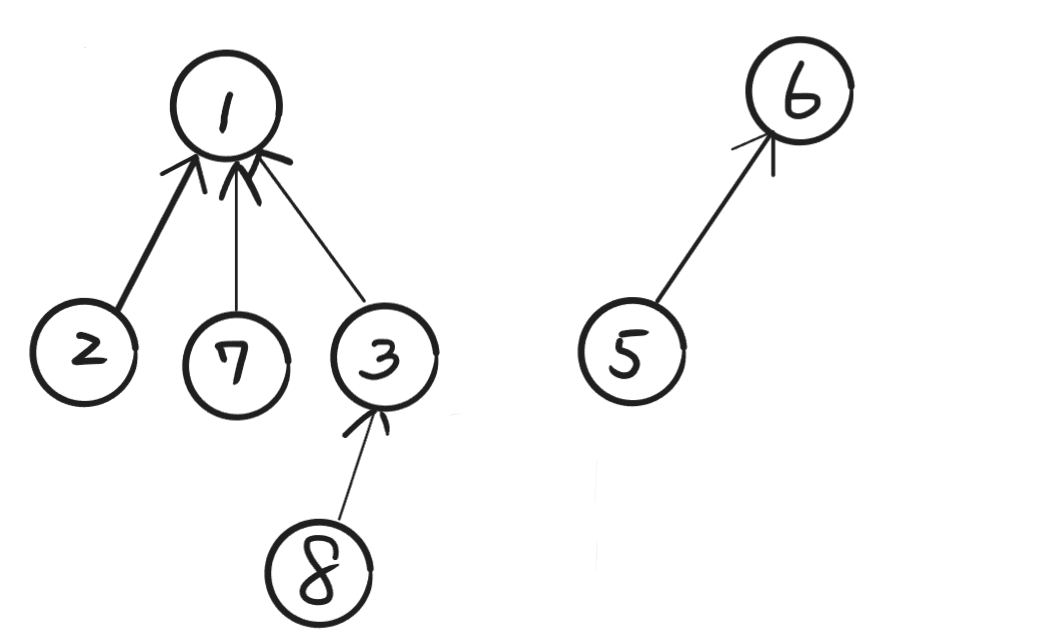
\includegraphics[width=\textwidth]{../Images/DSU.png}
        \caption{並查集示意圖}
    \end{figure}

    \textbf{合併}

    合併兩個組別(a,b)非常簡單,我們只要將節點a的頂,與節點b的頂結合就可以了,也就是說,
    將a的頂設為b的頂的上面,或是反過來,都可以完成。

    \subsection{啟發式合併}
    啟發式合併藉由將大的集合的頂,設在小的集合上面,以增進運行效率。原本沒有啟發式合併的並查集,
    期望複雜度為$O(n)$,加上啟發式合併之後可以降到$O(\log{(n)})$。

    \subsection{路徑壓縮}
    如果我們在查詢的時候,將所有經過的節點直接連上最頂的那一個,我們可以進一步改善複雜度到平均
    $O(\alpha(n))$,在競賽中可以視為常數$4$。

    \subsection{實作}
    實作上,因為通常加上路徑壓縮就足以勝任大部分任務,所以我們可以省略啟發式合併。

\begin{lstlisting}[caption=DSU 實作]
const int N=100010;
int dsu[N];

int find(int a){
    if(dsu[a]==a){
        return a;
    }
    // 路徑壓縮
    return dsu[a]=find(dsu[a]);
}

int Union(int a,int b){
    dsu[find(a)]=dsu[find(b)];
}
\end{lstlisting}

    \subsection{範例與練習}

    \problem 請實作啟發式合併。

    \problem UVA793 A - Network Connections

    \textbf{題目敘述}

    有$n$台電腦,編號為$1$至$n$,接下來有若干個指令,指令為\verb|c a b|代表連接$a$和$b$,
    指令為\verb|q a b|代表詢問$a$與$b$是否相連,最後請輸出總共有幾次詢問是得到「相連」的答案,
    以及總共有幾次詢問是得到「不相連」的答案。

    \textbf{範例測試}

    \begin{tabular}{|m{7cm}|m{7cm}|}
        \hline
        範例輸入 1 & 範例輸出 1 \\
        \hline
        \verb|10|    & \verb|1,2| \\
        \verb|c 1 5| & \\
        \verb|c 2 7| & \\
        \verb|q 7 1| & \\
        \verb|c 3 9| & \\
        \verb|q 9 6| & \\
        \verb|c 2 5| & \\
        \verb|q 7 5| & \\
        \hline
    \end{tabular}

    \textbf{小小細節}

    UVA因為很老,有一些奇怪的規定,例如最後一行不要換行等等,總之要遵守才會得到$AC$。

    \problem ZJ d831 畢業旅行

    \textbf{題目敘述}

    多年來友情的羈絆,終於將在這畢業的季節開花結果。

    這幾天,班上同學們無時無刻都熱烈討論著畢業旅行的地點。
    小明說,如果要去六福村,可以順便去小人國;小美說,如果去了恆春的話,墾丁就在幾十公里外了,一定也要去玩;
    小華表示,小鬼湖跟大鬼湖好像很近,似乎都是很有趣的地方。

    身為班長,聽到同學這麼多「去了哪裡也可以去哪裡」的資訊後,
    你決定要為班上的同學們,找到一個能玩最多景點的畢業旅行。

    \textbf{輸入說明}

    有多組測試資料,以 EOF 結束。

    每組測試資料的第一行有兩個正整數 $n (n \le 10^6)$ 和 $m (m \le 10^5)$,
    表示景點有 $n$ 個,編號為 $0 - (n-1)$。
    接下來有 $m$ 行,每行有兩個整數 $a$ 和 $b \; (0 \le a,b<n)$,
    表示去了 $a$ 的同時也可以去 $b$(反過來也一樣)。
    
    \textbf{輸出說明}

    輸出一個數字,表示畢業旅行最多可以玩的景點數量。

    \textbf{範例測試}

    \begin{tabular}{|m{7cm}|m{7cm}|}
        \hline
        範例輸入 1 & 範例輸出 1 \\
        \hline
        \verb|6 4| & \verb|4| \\
        \verb|0 1| & \verb|1| \\
        \verb|2 3| & \verb|2| \\
        \verb|1 3| & \\
        \verb|5 4| & \\
        \verb|1000000 0| & \\
        \verb|1000000 1| & \\
        \verb|0 999999| & \\
        \hline
    \end{tabular}

    \problem 洛谷P1536 村村通

    \textbf{題目敘述}

    某市調查城鎮交通狀況,得到現有城鎮道路統計表。
    表中列出了每條道路直接連通的城鎮。
    市政府「村村通工程」的目標是使全市任何兩個城鎮間都可以實現交通(但不一定有直接的道路相連,只要相互之間可達即可)。
    請你計算出最少還需要建設多少條道路?

    \textbf{輸入說明}

    輸入包含若干組測試數據,每組測試數據的第一行給出兩個用空格隔開的正整數,分別是城鎮數目 $n$ 和道路數目 $m$ ;隨後的 $m$ 行對應 $m$ 條道路,每行給出一對用空格隔開的正整數,分別是該條道路直接相連的兩個城鎮的編號。簡單起見,城鎮從 $1$ 到 $n$ 編號。

    注意:兩個城市間可以有多條道路相通。

    在輸入數據的最後,為一行一個整數 $0$,代表測試數據的結尾。
    
    \textbf{輸出說明}

    對於每組數據,對應一行一個整數。表示最少還需要建設的道路數目。

    \textbf{範例測試}

    \begin{tabular}{|m{7cm}|m{7cm}|}
        \hline
        範例輸入 1 & 範例輸出 1 \\
        \hline
        \verb|4 2| & \verb|1| \\
        \verb|1 3| & \verb|0| \\
        \verb|4 3| & \verb|2| \\
        \verb|3 3| & \verb|998| \\
        \verb|1 2| & \\
        \verb|1 3| & \\
        \verb|2 3| & \\
        \verb|5 2| & \\
        \verb|1 2| & \\
        \verb|3 5| & \\
        \verb|999 0| & \\
        \verb|0| & \\
        \hline
    \end{tabular}